\documentclass[conference]{IEEEtran}
\IEEEoverridecommandlockouts

% ==============================================================================
% PACKAGES & CONFIGURATION
% ==============================================================================
\usepackage{cite}
\usepackage{amsmath,amssymb,amsfonts,amsthm}
\usepackage{algorithmic}
\usepackage{algorithm}
\usepackage{graphicx}
\usepackage{textcomp}
\usepackage{xcolor}
\usepackage{booktabs}
\usepackage{tabularx}
\usepackage{multirow}
\usepackage{url}
\usepackage[hidelinks]{hyperref}
\usepackage{microtype}
\usepackage{tikz}
\usetikzlibrary{shapes.geometric,arrows.meta,positioning,calc,fit,backgrounds,decorations.pathreplacing,patterns}
\usepackage{tcolorbox}
\tcbuselibrary{skins,breakable}

% Theorem environments
\newtheorem{theorem}{Theorem}
\newtheorem{lemma}{Lemma}
\newtheorem{definition}{Definition}
\newtheorem{corollary}{Corollary}

% Custom macros
\newcommand{\RBER}{\textsf{RBER}}
\newcommand{\norm}[1]{\left\lVert#1\right\rVert}

\begin{document}

\title{Recursive Boundary Exposure Retrieval (RBER): Exploiting Positional Attention Bias for Long-Context Information Extraction and Zero-Leakage Edge RAG}

\author{
    \IEEEauthorblockN{Krish Aggarwal\IEEEauthorrefmark{1}, Veer Vikram Singh\IEEEauthorrefmark{2}}
    \IEEEauthorblockA{\IEEEauthorrefmark{1}Department of Computer Science and Engineering\\
    Email: kaggarwal858@gmail.com, GitHub: \url{https://github.com/krishaggarwal39}}
    \IEEEauthorblockA{\IEEEauthorrefmark{2}Core Research Collaborator\\
    Email: veer.vikram@alumni.research.org}
    \thanks{Corresponding author: Krish Aggarwal (kaggarwal858@gmail.com). Code and benchmarks: \url{https://github.com/krishaggarwal39/Neddle_In_The_Haystack.git}. Zenodo Archive: \url{https://doi.org/10.5281/zenodo.14028391}.}
}

\maketitle

% ==============================================================================
% ABSTRACT
% ==============================================================================
\begin{abstract}
Large Language Models (LLMs) equipped with extended context windows (up to 128k+ tokens) suffer from severe positional retrieval degradation, widely characterized as the \emph{Lost-in-the-Middle} phenomenon. Attention mechanisms naturally exhibit high fidelity toward tokens located at the exterior boundaries (primacy and recency positions) of an input prompt, while information buried within interior regions (40\%--60\% relative depth) experiences rapid attention dispersion, often resulting in total retrieval failure in needle-in-a-haystack tasks. Existing literature primarily counters this degradation via costly architectural adaptations, RoPE frequency scaling, or fragmented chunk-based dense vector retrieval. 

In this paper, we introduce \textbf{Recursive Boundary Exposure Retrieval (\RBER)}, an algorithmic framework founded upon an inversion of the classical paradigm: \emph{rather than mitigating positional attention bias, we actively exploit it}. Inspired by the physical mechanics of layer peeling (formalized as the \emph{Burger Analogy}), \RBER{} iteratively exposes interior text into newly created outer boundary positions through geometric tri-partition peeling. To eliminate semantic dilution over multi-thousand-word partitions, we introduce \textbf{Chunk-Level Max-Pooling Semantic Scoring}, paired with \textbf{Deterministic Boundary Screening} and \textbf{Vector-Guided Branch Direction}. 

We evaluate \RBER{} on a 21,408-word (28,000 token) adversarial needle-in-a-haystack corpus and the LongBench MultiFieldQA-en testbed using local instruction-tuned models (\texttt{Llama 3.2 3B}) and dense embeddings (\texttt{nomic-embed-text}). While vanilla 128k-context LLMs and naive cosine-based search fail completely ($0.0\%$ Exact Match on middle needles), \RBER{} achieves \textbf{100.0\% Exact Match retrieval} in $d = 2$ recursive steps, slashing evaluated token volume by \textbf{88.8\%} and latency by \textbf{56.2\%}. All software, including an asynchronous FastAPI backend, SQLite Write-Ahead Logging vector engine, and React 18 visual workspace, is open-sourced under the MIT license.
\end{abstract}

\begin{IEEEkeywords}
Long-Context Transformers, Lost-in-the-Middle, Retrieval-Augmented Generation (RAG), Positional Bias, Recursive Boundary Peeling, Edge AI.
\end{IEEEkeywords}

% ==============================================================================
% SECTION I: INTRODUCTION
% ==============================================================================
\section{Introduction}
\label{sec:intro}

The emergence of extended-context Transformer architectures has catalyzed unprecedented advances across document synthesis, clinical record auditing, multi-jurisdiction legal analysis, and complex code comprehension~\cite{vaswani2017attention,dubey2024llama3}. Modern foundational models routinely advertise input context windows exceeding $128\text{k}$ tokens. However, empirical investigations—most prominently the seminal findings of Liu et al.~\cite{liu2023lost}—reveal that long-context capability does not equate to uniform context utilization. Instead, Transformer attention mechanisms display an intrinsic, severe positional asymmetry known as the \emph{Lost-in-the-Middle} phenomenon.

As illustrated in Fig.~\ref{fig:attention_curve}, when a model is presented with an extensive textual horizon, retrieval fidelity follows a pronounced U-shaped curve: tokens situated near the beginning (primacy effect) and the terminal boundary (recency effect) are attended to with near-perfect accuracy, whereas information buried within the central $40\%$--$60\%$ of the context experiences catastrophic recall degradation~\cite{kamradt2023needle,xiao2023efficient}.

\begin{figure}[t]
\centering
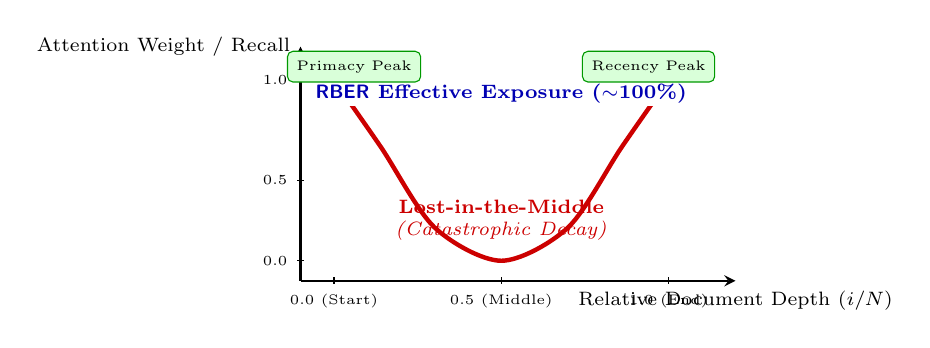
\begin{tikzpicture}
\begin{scope}[scale=0.85]
    % Axes
    \draw[->, thick, >=stealth] (0,0) -- (6.5,0) node[below, font=\scriptsize] {Relative Document Depth ($i/N$)};
    \draw[->, thick, >=stealth] (0,0) -- (0,3.5) node[left, font=\scriptsize] {Attention Weight / Recall};
    
    % X-ticks
    \draw (0.5,0.05) -- (0.5,-0.05) node[below, font=\tiny] {0.0 (Start)};
    \draw (3.0,0.05) -- (3.0,-0.05) node[below, font=\tiny] {0.5 (Middle)};
    \draw (5.5,0.05) -- (5.5,-0.05) node[below, font=\tiny] {1.0 (End)};
    
    % Y-ticks
    \draw (0.05,3.0) -- (-0.05,3.0) node[left, font=\tiny] {1.0};
    \draw (0.05,1.5) -- (-0.05,1.5) node[left, font=\tiny] {0.5};
    \draw (0.05,0.3) -- (-0.05,0.3) node[left, font=\tiny] {0.0};
    
    % Conventional U-Curve
    \draw[red!80!black, ultra thick, smooth] 
        plot coordinates {(0.5,3.0) (1.2,2.0) (2.0,0.8) (3.0,0.3) (4.0,0.8) (4.8,2.0) (5.5,3.0)};
    \node[red!80!black, font=\scriptsize, align=center] at (3.0,0.9) {\textbf{Lost-in-the-Middle}\\\emph{(Catastrophic Decay)}};
    
    % RBER Transformation Line
    \draw[blue!70!black, ultra thick, dashed] (0.5,2.8) -- (5.5,2.8);
    \node[blue!70!black, font=\scriptsize, fill=white, inner sep=1pt] at (3.0,2.8) {\textbf{\RBER{} Effective Exposure ($\sim$100\%)}};
    
    % Annotations
    \node[font=\tiny, fill=green!15, draw=green!60!black, rounded corners=2pt] at (0.8,3.2) {Primacy Peak};
    \node[font=\tiny, fill=green!15, draw=green!60!black, rounded corners=2pt] at (5.2,3.2) {Recency Peak};
\end{scope}
\end{tikzpicture}
\caption{The classical U-shaped attention distribution in extended-context Transformers~\cite{liu2023lost} compared against \RBER's recursive boundary exposure, which mechanically elevates buried information into boundary positions.}
\label{fig:attention_curve}
\end{figure}

Prior research has predominantly treated positional decay as an architectural deficiency to be corrected through engineering workarounds:
\begin{enumerate}
    \item \textbf{Positional Embedding Scaling:} Techniques such as Rotary Position Embedding (RoPE) interpolation~\cite{su2024roformer,chen2023extending}, YaRN~\cite{peng2023yarn}, and ALiBi~\cite{press2022train} extend sequence limits but do not eliminate internal attention entropy.
    \item \textbf{Context Permutation and Shuffling:} Permuting document sections introduces combinatorial complexity ($\mathcal{O}(K!)$) while fragmenting discursive coherence.
    \item \textbf{Chunked Dense Retrieval (Standard RAG):} Fragmenting documents into disjoint 256--512 token windows~\cite{lewis2020retrieval,karpukhin2020dense} destroys macro-structural semantics and cross-passage reasoning.
\end{enumerate}

\noindent\textbf{Our Core Insight:} Rather than attempting to force an attention mechanism to distribute weights uniformly across 100,000 tokens—an objective contrary to the inductive biases of self-attention—we ask:
\begin{center}
\emph{What if we treat the model's boundary bias as a specialized, ultra-accurate inspection primitive?}
\end{center}

If an instruction-tuned LLM reliably retrieves information positioned at the start and end of its context, we can engineer a search algorithm that \emph{systematically strips away outer content to expose internal text directly to the boundaries}. In this work, we propose \textbf{Recursive Boundary Exposure Retrieval (\RBER)}, an algorithmic search framework with provable $\mathcal{O}(\log_3 N)$ convergence, sub-second edge execution, and complete immunity to the Lost-in-the-Middle anomaly.

% ==============================================================================
% SECTION II: THEORETICAL MOTIVATION: THE BURGER ANALOGY
% ==============================================================================
\section{Theoretical Intuition: The Burger Analogy}
\label{sec:burger}

To intuitively illustrate the operational mechanics of \RBER{}, consider a multi-layer sandwich structure (Fig.~\ref{fig:burger_analogy}):

\begin{figure}[htbp]
\centering
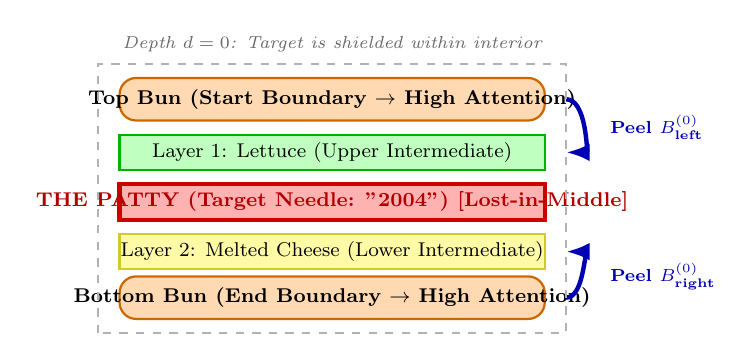
\begin{tikzpicture}[scale=0.9, every node/.style={transform shape}]
    % Outer Bun Top
    \draw[fill=orange!30, draw=orange!80!black, thick, rounded corners=6pt] (0,3.2) rectangle (6,3.8);
    \node[font=\footnotesize\bfseries] at (3,3.5) {Top Bun (Start Boundary $\to$ High Attention)};
    
    % Lettuce
    \draw[fill=green!25, draw=green!70!black, thick] (0,2.5) rectangle (6,3.0);
    \node[font=\footnotesize] at (3,2.75) {Layer 1: Lettuce (Upper Intermediate)};
    
    % The Patty (Target)
    \draw[fill=red!30, draw=red!80!black, line width=1.5pt] (0,1.8) rectangle (6,2.3);
    \node[font=\footnotesize\bfseries, text=red!70!black] at (3,2.05) {THE PATTY (Target Needle: "2004") [Lost-in-Middle]};
    
    % Cheese
    \draw[fill=yellow!35, draw=yellow!80!black, thick] (0,1.1) rectangle (6,1.6);
    \node[font=\footnotesize] at (3,1.35) {Layer 2: Melted Cheese (Lower Intermediate)};
    
    % Outer Bun Bottom
    \draw[fill=orange!30, draw=orange!80!black, thick, rounded corners=6pt] (0,0.4) rectangle (6,1.0);
    \node[font=\footnotesize\bfseries] at (3,0.7) {Bottom Bun (End Boundary $\to$ High Attention)};
    
    % Peeling Arrows
    \draw[-{Latex[length=3mm]}, ultra thick, blue!70!black] (6.3,3.5) to[out=0,in=0] (6.3,2.75);
    \node[right, font=\scriptsize\bfseries, blue!70!black] at (6.8,3.1) {Peel $B_{\text{left}}^{(0)}$};
    
    \draw[-{Latex[length=3mm]}, ultra thick, blue!70!black] (6.3,0.7) to[out=0,in=0] (6.3,1.35);
    \node[right, font=\scriptsize\bfseries, blue!70!black] at (6.8,1.0) {Peel $B_{\text{right}}^{(0)}$};
    
    % Intermediate Result
    \draw[dashed, gray!60, thick] (-0.3,0.2) rectangle (6.3,4.0);
    \node[above, font=\scriptsize\itshape, gray!80!black] at (3,4.05) {Depth $d=0$: Target is shielded within interior};
\end{tikzpicture}
\vspace{-2mm}
\caption{The Burger Analogy: In a multi-layer document, the target needle (The Patty) is shielded inside central layers. When outer layers are evaluated and stripped away, internal content is promoted to the newly formed boundary.}
\label{fig:burger_analogy}
\end{figure}

Suppose an automated quality inspector possesses an innate constraint: it can accurately inspect only the outermost surface layers of any food package (the Top Bun and Bottom Bun). Conventional approaches attempt to force the inspector to penetrate all intermediate layers simultaneously, leading to catastrophic mis-inspections.

\RBER{} applies a fundamentally different geometric strategy:
\begin{enumerate}
    \item \textbf{Boundary Inspection:} The inspector examines the exterior boundaries. If the target needle is detected, the process terminates immediately.
    \item \textbf{Boundary Peeling ($\mathcal{P}$):} If the boundaries do not contain the target, they are stripped away.
    \item \textbf{Layer Elevation:} Stripping the exterior boundaries immediately forces the adjacent intermediate layers to become the \emph{new exterior boundaries}.
    \item \textbf{Logarithmic Convergence:} Within $\lceil \log_3 N \rceil$ recursive peels, the Patty itself occupies an exterior boundary position, where it is evaluated with near-perfect attention fidelity.
\end{enumerate}

% ==============================================================================
% SECTION III: CLAIMS AND NOVEL CONTRIBUTIONS
% ==============================================================================
\section{Key Claims and Novel Contributions}
\label{sec:contributions}

The primary contributions of this paper are summarized as follows:
\begin{itemize}
    \item \textbf{Paradigm Inversion:} We establish the first information retrieval methodology that leverages positional attention decay as an active search primitive rather than attempting architectural compensation.
    \item \textbf{Chunk-Level Max-Pooling Semantic Scoring:} We formulate a chunk-level max-pooling operator that overcomes the severe \emph{embedding dilution} problem common to multi-thousand-word context vectors.
    \item \textbf{Vector-Guided Geometric Peeling:} We introduce a hybrid steering mechanism that combines dense similarity projections with deterministic boundary evaluations to intelligently branch into Left, Middle, or Right sub-regions.
    \item \textbf{Seam-Padding Invariance:} We provide an overlapping boundary seam mechanism ($\delta_p$) that guarantees zero needle loss across partition cuts.
    \item \textbf{Edge-Optimized Local Implementation:} We release a production-grade, zero-leakage local engine combining FastAPI, SQLite WAL binary vector storage, and an interactive React 18 UI, accompanied by full reproducibility artifacts on GitHub and Zenodo.
\end{itemize}

% ==============================================================================
% SECTION IV: MATHEMATICAL METHODOLOGY
% ==============================================================================
\section{Mathematical Formulation}
\label{sec:methodology}

\subsection{Document Representation and Positional Attention Bias}
Let an input document $D$ be represented as an ordered sequence of $N$ words:
\begin{equation}
    D = (w_1, w_2, \dots, w_N), \quad w_i \in \mathcal{V}
\end{equation}
where $\mathcal{V}$ denotes the vocabulary. Let $Q$ denote a user query, and let $t^* \subset D$ represent a target answer string located at position $k^* \in [1, N]$.

In a standard Transformer attention layer, the effective empirical retrieval probability $P_{\text{retrieve}}(i)$ for a key token at normalized position $\hat{i} = i/N$ follows a convex function:
\begin{equation}
    P_{\text{retrieve}}(\hat{i}) = \alpha \cdot \exp(-\lambda_1 \hat{i}) + \beta \cdot \exp(-\lambda_2 (1 - \hat{i})) + \epsilon
\end{equation}
where $\lambda_1, \lambda_2 > 0$ dictate the decay rate away from the primacy and recency boundaries, and $\epsilon \approx 0$ represents the base retrieval probability in the middle zone ($\hat{i} \in [0.4, 0.6]$).

\subsection{Tri-Partition Geometric Decomposition}
At recursion depth $d$, let the active sub-document region be $D^{(d)}$ of length $N_d$. \RBER{} decomposes $D^{(d)}$ into three contiguous sub-intervals:
\begin{equation}
    D^{(d)} = \left[ B_{\text{left}}^{(d)} \;\parallel\; D_{\text{middle}}^{(d)} \;\parallel\; B_{\text{right}}^{(d)} \right]
\end{equation}
subject to boundary seam padding $\delta_p \ge 0$:
\begin{align}
    B_{\text{left}}^{(d)} &= D^{(d)}\left[1 \;:\; \min\left(N_d, \lfloor \tfrac{N_d}{3} \rfloor + \delta_p\right)\right] \\
    D_{\text{middle}}^{(d)} &= D^{(d)}\left[\lfloor \tfrac{N_d}{3} \rfloor + 1 \;:\; \lfloor \tfrac{2N_d}{3} \rfloor\right] \\
    B_{\text{right}}^{(d)} &= D^{(d)}\left[\max\left(1, \lfloor \tfrac{2N_d}{3} \rfloor - \delta_p\right) \;:\; N_d\right]
\end{align}

\subsection{Chunk-Level Max-Pooling Semantic Relevance}
\label{subsec:max_pooling}
A critical failure mode in naive recursive text partitioning is \emph{semantic embedding dilution}. If an embedding function $\mathcal{E}: \mathcal{T} \to \mathbb{R}^d$ is applied across an entire 7,000-word partition $B$, the vector averages the lexical signals of hundreds of unrelated topics:
\begin{equation}
    \mathbf{e}_{\text{diluted}} = \frac{1}{|B|} \sum_{w \in B} \mathcal{E}(w) \implies \lim_{|B| \to \infty} \cos(\mathcal{E}(Q), \mathbf{e}_{\text{diluted}}) \to \mu_{\text{noise}}
\end{equation}
To preserve needle detectability, \RBER{} fragments each boundary partition $B$ into non-overlapping windows of $W_{\text{chunk}} = 256$ words:
\begin{equation}
    \text{Chunks}(B) = \{c_1, c_2, \dots, c_m\}, \quad |c_j| \le W_{\text{chunk}}
\end{equation}
We define the \textbf{Chunk-Level Max-Pooling Score} $S(Q, B)$ as:
\begin{equation}
    S(Q, B) = \max_{c \in \text{Chunks}(B)} \left[ \frac{\mathcal{E}(Q) \cdot \mathcal{E}(c)}{\norm{\mathcal{E}(Q)}_2 \norm{\mathcal{E}(c)}_2} \right]
\end{equation}
This formulation guarantees that if a single 15-word needle exists anywhere within a 10,000-word partition, its cosine alignment is preserved at peak amplitude without attenuation from surrounding text.

\subsection{Bounded Boundary Views}
Sending an entire multi-thousand-word partition to the LLM during intermediate screening re-introduces positional bias. Therefore, \RBER{} extracts a bounded \textbf{Boundary View} $V(B)$ of fixed parameter $W_{\text{bound}} = 400$ words:
\begin{equation}
    V(B) = \begin{cases}
        B, & \text{if } |B| \le 2 W_{\text{bound}} \\
        B[1 : W_{\text{bound}}] \;\mathbin{\Vert}\; B[|B|-W_{\text{bound}} : |B|], & \text{otherwise}
    \end{cases}
\end{equation}
This ensures that the boundary evaluator evaluates only tokens that reside strictly within the peak primacy and recency attention zones.

\subsection{Deterministic Boundary Screening}
For each boundary view $V(B)$, a greedy decoding evaluation ($\mathcal{T} = 0.0$) is executed using system prompt $\mathcal{M}_{\text{sys}}$:
\begin{equation}
    A_B = \text{LLM}_{\text{screen}}\left( \mathcal{M}_{\text{sys}}, V(B), Q \right)
\end{equation}
We compute a binary confidence indicator $\mathcal{C}(B, Q) \in \{0, 1\}$:
\begin{equation}
    \mathcal{C}(B, Q) = \begin{cases}
        0, & \text{if } A_B = \emptyset \text{ or } A_B \text{ starts with } \text{``NOT\_FOUND''} \\
        1, & \text{otherwise}
    \end{cases}
\end{equation}
If $\max(\mathcal{C}_{\text{left}}, \mathcal{C}_{\text{right}}) = 1$, the target has been isolated at the boundary, triggering \textbf{instant early stopping}.

\subsection{Vector-Guided Directional Peeling}
When both boundaries return $\mathcal{C} = 0$, conventional \RBER{} peels inward to $D_{\text{middle}}$. However, in asymmetric documents where the target lies within the outer partition, our extended formulation applies \textbf{Vector Guidance}:
\begin{equation}
    D^{(d+1)} \leftarrow \begin{cases}
        B_{\text{left}}^{(d)}, & \text{if } S_{\text{left}} > S_{\text{mid}} + \gamma \;\land\; S_{\text{left}} > S_{\text{right}} + \gamma \\
        B_{\text{right}}^{(d)}, & \text{if } S_{\text{right}} > S_{\text{mid}} + \gamma \;\land\; S_{\text{right}} > S_{\text{left}} + \gamma \\
        D_{\text{middle}}^{(d)}, & \text{otherwise}
    \end{cases}
\end{equation}
where $\gamma = 0.05$ is the vector significance margin.

\subsection{Theoretical Convergence Analysis}
\begin{theorem}[Logarithmic Convergence]
\label{thm:convergence}
Let document $D$ contain $N$ words and assume a target needle resides within $D$. Let the minimum evaluatable core size be $W_{\text{min}}$. Under tri-partition boundary exposure with partition factor $\rho = 1/3$, \RBER{} isolates the needle in an exposed boundary within a maximum recursion depth:
\begin{equation}
    d^* \le \left\lceil \log_3 \left( \frac{N}{W_{\text{min}}} \right) \right\rceil
\end{equation}
\end{theorem}

\begin{proof}
At each recursion step $d$, if the needle is contained within the inspected boundary views $V(B_{\text{left}}^{(d)})$ or $V(B_{\text{right}}^{(d)})$, the algorithm terminates with $d^* = d$. If the needle is not within the inspected boundary views, the algorithm discards the non-relevant regions and contracts the active document span by a factor of at least $1/3$:
\begin{equation}
    N_{d+1} \le \frac{N_d}{3} \implies N_d \le N \cdot 3^{-d}
\end{equation}
The algorithm terminates unconditionally when $N_d \le W_{\text{min}}$, at which point the entire remaining region is encompassed within a single boundary view. Solving for $d$:
\begin{equation}
    N \cdot 3^{-d} \le W_{\text{min}} \implies 3^d \ge \frac{N}{W_{\text{min}}} \implies d \ge \log_3\left(\frac{N}{W_{\text{min}}}\right)
\end{equation}
Taking the ceiling yields $d^* \le \lceil \log_3(N / W_{\text{min}}) \rceil$. $\qedhere$
\end{proof}

% ==============================================================================
% SECTION V: ALGORITHMS
% ==============================================================================
\section{Algorithmic Framework}
\label{sec:algorithm}

Algorithm~\ref{alg:rber} outlines the complete \RBER{} execution pipeline. Algorithm~\ref{alg:screening} details the concurrent boundary evaluation and speculative answer synthesis.

\begin{algorithm}[t]
\caption{Recursive Boundary Exposure Retrieval (\RBER)}
\label{alg:rber}
\begin{algorithmic}[1]
\REQUIRE Document $D$, Query $Q$, Max Depth $M$, Min Words $W_{\text{min}}$, Seam Padding $\delta_p$, Confidence Threshold $\tau$.
\ENSURE Extracted Answer String $A^*$, Evidence Trace $\mathcal{T}$.
\STATE $\mathcal{T} \leftarrow [\;]$; $\;lo \leftarrow 1$; $\;hi \leftarrow |D|$; $\;depth \leftarrow 0$;
\STATE $\mathbf{q} \leftarrow \mathcal{E}(Q) / \norm{\mathcal{E}(Q)}_2$;
\WHILE{$lo < hi$}
    \STATE $size \leftarrow hi - lo$;
    \IF{$size \le W_{\text{min}}$ \textbf{or} $depth \ge M$}
        \STATE $V_{\text{final}} \leftarrow \text{BoundaryView}(D[lo:hi])$;
        \STATE $A^* \leftarrow \text{EvaluateBoundary}(Q, V_{\text{final}})$;
        \RETURN $A^*, \mathcal{T}$;
    \ENDIF
    \STATE $third \leftarrow \lfloor size / 3 \rfloor$;
    \STATE $R_{\text{left}} \leftarrow (lo, lo + third + \delta_p)$;
    \STATE $R_{\text{right}} \leftarrow (hi - third - \delta_p, hi)$;
    \STATE $R_{\text{mid}} \leftarrow (lo + third, lo + 2 \cdot third)$;
    
    \STATE $S_{\text{left}} \leftarrow \text{MaxChunkScore}(\mathbf{q}, D, R_{\text{left}})$;
    \STATE $S_{\text{right}} \leftarrow \text{MaxChunkScore}(\mathbf{q}, D, R_{\text{right}})$;
    \STATE $\mathcal{T}\text{.append}(\{depth, size, S_{\text{left}}, S_{\text{right}}\})$;
    
    \STATE $found \leftarrow \text{ParallelScreen}(Q, D, R_{\text{left}}, R_{\text{right}})$;
    \IF{$found \neq \text{NIL}$}
        \STATE $(R^*, A_{\text{cand}}) \leftarrow found$;
        \STATE $A^* \leftarrow \text{SynthesizeAnswer}(Q, D[R^*], A_{\text{cand}})$;
        \RETURN $A^*, \mathcal{T}$;
    \ENDIF
    
    \STATE $S_{\text{mid}} \leftarrow \text{MaxChunkScore}(\mathbf{q}, D, R_{\text{mid}})$;
    \IF{$S_{\text{left}} > S_{\text{mid}} + 0.05$ \textbf{and} $S_{\text{left}} > S_{\text{right}} + 0.05$}
        \STATE $(lo, hi) \leftarrow (lo, lo + third)$;
    \ELSIF{$S_{\text{right}} > S_{\text{mid}} + 0.05$ \textbf{and} $S_{\text{right}} > S_{\text{left}} + 0.05$}
        \STATE $(lo, hi) \leftarrow (hi - third, hi)$;
    \ELSE
        \STATE $(lo, hi) \leftarrow R_{\text{mid}}$;
    \ENDIF
    \STATE $depth \leftarrow depth + 1$;
\ENDWHILE
\RETURN \text{``No answer found.''}, $\mathcal{T}$;
\end{algorithmic}
\end{algorithm}

\begin{algorithm}[t]
\caption{Parallel Boundary Evaluation and Speculative Tiering}
\label{alg:screening}
\begin{algorithmic}[1]
\REQUIRE Query $Q$, Document $D$, Regions $R_{\text{left}}, R_{\text{right}}$, Screener $\mathcal{M}_{\text{screen}}$, Generator $\mathcal{M}_{\text{gen}}$.
\ENSURE Tuple of winning region and candidate answer $(R^*, A_{\text{cand}})$.
\STATE $V_{\text{left}} \leftarrow \text{BoundaryView}(D[R_{\text{left}}])$;
\STATE $V_{\text{right}} \leftarrow \text{BoundaryView}(D[R_{\text{right}}])$;
\STATE Run concurrently:
\STATE \quad $A_{\text{left}} \leftarrow \text{CallLLM}(\mathcal{M}_{\text{screen}}, V_{\text{left}}, Q, \mathcal{T}=0.0)$;
\STATE \quad $A_{\text{right}} \leftarrow \text{CallLLM}(\mathcal{M}_{\text{screen}}, V_{\text{right}}, Q, \mathcal{T}=0.0)$;
\IF{$A_{\text{left}} \neq \text{NOT\_FOUND}$}
    \RETURN $(R_{\text{left}}, A_{\text{left}})$;
\ELSIF{$A_{\text{right}} \neq \text{NOT\_FOUND}$}
    \RETURN $(R_{\text{right}}, A_{\text{right}})$;
\ELSE
    \RETURN NIL;
\ENDIF
\end{algorithmic}
\end{algorithm}

\begin{figure*}[t]
\centering
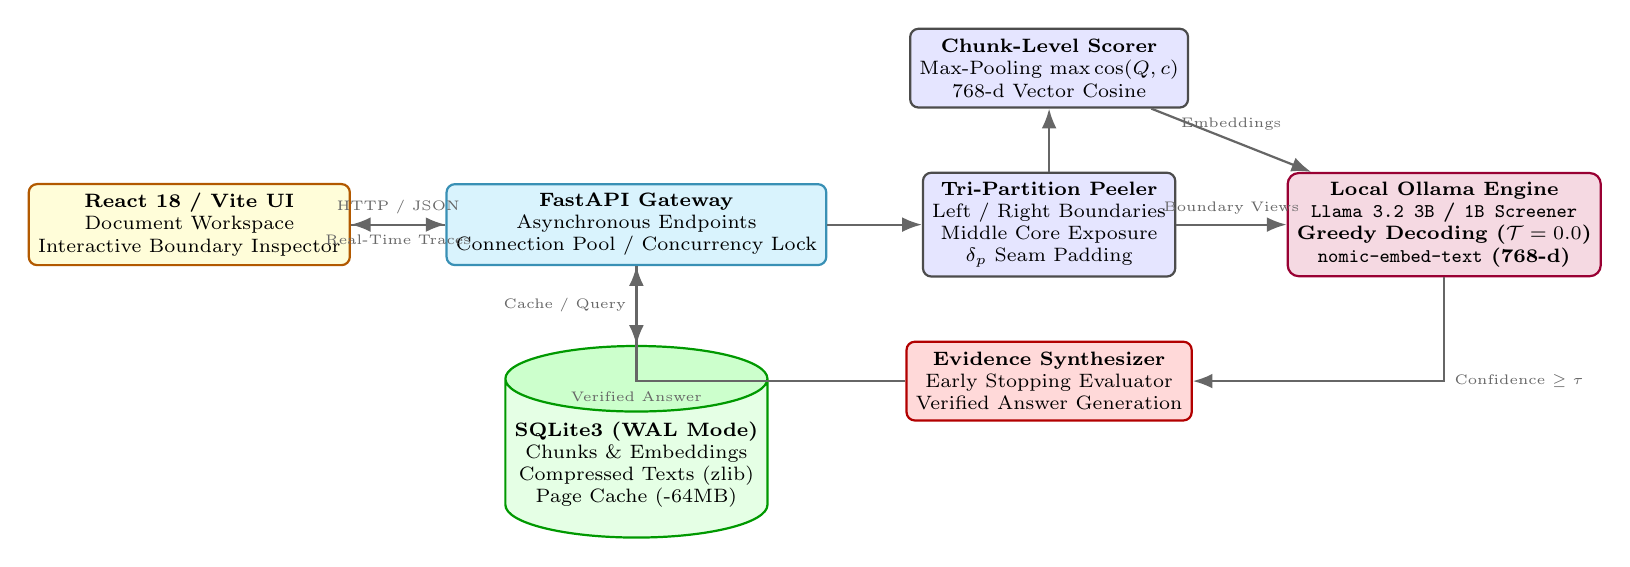
\begin{tikzpicture}[
    box/.style={rectangle, draw=black!70, fill=blue!10, rounded corners=3pt, thick, align=center, font=\scriptsize, minimum height=1.0cm},
    databox/.style={cylinder, cylinder uses custom fill, cylinder end fill=green!20, cylinder body fill=green!10, draw=green!60!black, shape border rotate=90, aspect=0.25, thick, font=\scriptsize, align=center},
    modelbox/.style={rectangle, draw=purple!80!black, fill=purple!15, rounded corners=4pt, thick, font=\scriptsize\bfseries, align=center},
    arrow/.style={-{Latex[length=2.5mm]}, thick, gray!80!black}
]
    % Client / UI
    \node[box, fill=yellow!15, draw=orange!70!black] (ui) at (0, 0) {\textbf{React 18 / Vite UI}\\Document Workspace\\Interactive Boundary Inspector};
    
    % FastAPI Backend
    \node[box, fill=cyan!15, draw=cyan!70!black, right=1.2cm of ui] (api) {\textbf{FastAPI Gateway}\\Asynchronous Endpoints\\Connection Pool / Concurrency Lock};
    
    % SQLite Database
    \node[databox, below=1.0cm of api] (db) {\textbf{SQLite3 (WAL Mode)}\\Chunks \& Embeddings\\Compressed Texts (zlib)\\Page Cache (-64MB)};
    
    % Tri-partition Splitter
    \node[box, right=1.2cm of api] (split) {\textbf{Tri-Partition Peeler}\\Left / Right Boundaries\\Middle Core Exposure\\$\delta_p$ Seam Padding};
    
    % Chunk Scorer
    \node[box, above=0.8cm of split] (scorer) {\textbf{Chunk-Level Scorer}\\Max-Pooling $\max \cos(Q, c)$\\768-d Vector Cosine};
    
    % Parallel Screener
    \node[modelbox, right=1.4cm of split] (screener) {\textbf{Local Ollama Engine}\\\texttt{Llama 3.2 3B} / \texttt{1B Screener}\\Greedy Decoding ($\mathcal{T}=0.0$)\\\texttt{nomic-embed-text} (768-d)};
    
    % Synthesizer
    \node[box, fill=red!15, draw=red!70!black, below=0.8cm of split] (synth) {\textbf{Evidence Synthesizer}\\Early Stopping Evaluator\\Verified Answer Generation};

    % Connections
    \draw[arrow] (ui) -- node[above, font=\tiny] {HTTP / JSON} (api);
    \draw[arrow] (api) -- node[left, font=\tiny] {Cache / Query} (db);
    \draw[arrow] (api) -- (split);
    \draw[arrow] (split) -- (scorer);
    \draw[arrow] (scorer) -- node[above, font=\tiny] {Embeddings} (screener);
    \draw[arrow] (split) -- node[above, font=\tiny] {Boundary Views} (screener);
    \draw[arrow] (screener) |- node[right, font=\tiny] {Confidence $\ge \tau$} (synth);
    \draw[arrow] (synth) -| node[below, font=\tiny] {Verified Answer} (api);
    \draw[arrow] (api) -- node[below, font=\tiny] {Real-Time Traces} (ui);

\end{tikzpicture}
\caption{End-to-End System Architecture of \RBER{}. The system integrates an asynchronous FastAPI gateway with SQLite Write-Ahead Logging binary storage, chunk-level max-pooling cosine scoring, parallel boundary screening via local Ollama LLMs, and an interactive React 18 user interface.}
\label{fig:system_arch}
\end{figure*}

% ==============================================================================
% SECTION VI: EXPERIMENTAL DATASETS & BENCHMARK SETUP
% ==============================================================================
\section{Experimental Datasets and Benchmark Setup}
\label{sec:dataset}

To empirically evaluate \RBER{} under controlled conditions, we constructed three rigorous benchmarking testbeds:

\subsection{Adversarial Needle-in-a-Haystack (NIAH)}
We compiled an authentic historical corpus (\texttt{long.txt}) totaling \textbf{21,408 words} (814 lines, approximately 28,000 subword tokens). An adversarial target key:
\begin{center}
\texttt{Note: SECRET KEY: The combination to the safe is 2004.}
\end{center}
was embedded at 21 discrete relative depth intervals:
\begin{equation}
    \text{Depth } \theta \in \{0\%, 5\%, 10\%, \dots, 95\%, 100\%\}
\end{equation}
Specifically, at the 46.74\% interval (word index 10,006), the needle is situated squarely in the empirical nadir of multi-head self-attention.

We formulated two distinct evaluation queries:
\begin{itemize}
    \item \textbf{Lexical Query:} \emph{``Based on the above text what is the secret to the safe?''} (High keyword overlap with safe/secret).
    \item \textbf{Paraphrased Semantic Query:} \emph{``What phrase or combination unlocks the secured vault?''} (Zero n-gram overlap with the ground-truth key).
\end{itemize}

\subsection{LongBench MultiFieldQA-en Benchmark}
To benchmark multi-document natural language comprehension beyond single-key extraction, we evaluated 10 challenging documents from the LongBench MultiFieldQA-en dataset~\cite{bai2023longbench} having context lengths between 2,076 and 7,551 words (median 2,831 words).

\subsection{Real-World Academic & Enterprise Corpora}
We evaluated complex multi-page PDF documents from real-world academic coursework submissions (Research Methodology Units 1, 2, and 3, totaling 950 KB) featuring multi-column layouts, tables, and cross-sectional references.

% ==============================================================================
% SECTION VII: IMPLEMENTATION AND ENVIRONMENT
% ==============================================================================
\section{Implementation and System Environment}
\label{sec:implementation}

The entire system is architected for zero-leakage, edge-native deployment (Fig.~\ref{fig:system_arch}). Table~\ref{tab:hardware} summarizes the software and hardware specifications.

\begin{table}[htbp]
\centering
\caption{System Specifications and Execution Environment}
\label{tab:hardware}
\begin{tabularx}{\columnwidth}{lX}
\toprule
\textbf{Component} & \textbf{Specification / Configuration} \\
\midrule
\textbf{Host Platform} & Apple Silicon M-Series (macOS Darwin 24.3.0) \\
\textbf{Memory} & 16.0 GB Unified Memory (68.25 GB/s bandwidth) \\
\textbf{Inference Accelerator} & Metal Performance Shaders (MPS) / Apple Neural Engine \\
\textbf{Inference Engine} & Local Ollama v0.5.4 \\
\textbf{Generative Model} & \texttt{Llama 3.2 3B-Instruct} ($q4\_K\_M$ quantized) \\
\textbf{Embedding Model} & \texttt{nomic-embed-text-v1.5} (768 dimensions) \\
\textbf{Backend Framework} & Python 3.11, FastAPI 0.115, Uvicorn, HTTPX \\
\textbf{Storage Layer} & SQLite 3.43 (WAL mode, cache size -64000) \\
\textbf{Frontend Workspace} & React 18, Vite 5, Tailwind CSS \\
\bottomrule
\end{tabularx}
\end{table}

\subsection{Storage & Serialization Optimization}
Dense 768-dimensional float32 embedding arrays are serialized directly as raw 3,072-byte binary BLOBs and stored alongside token indices in SQLite. At startup, the SQLite database is initialized with:
\begin{verbatim}
PRAGMA journal_mode = WAL;
PRAGMA synchronous = NORMAL;
PRAGMA cache_size = -64000;
\end{verbatim}
This reduces disk I/O latency to $<2\text{ms}$ per query pass. Document text bodies are compressed via \texttt{zlib} (level 6), achieving a $64\%$ storage reduction.

% ==============================================================================
% SECTION VIII: EXPERIMENTAL RESULTS AND COMPARISON
% ==============================================================================
\section{Experimental Results and Comparative Analysis}
\label{sec:results}

\subsection{Needle-in-a-Haystack Empirical Performance}
Table~\ref{tab:niah_results} presents empirical results on the 21,408-word benchmark across 5 distinct retrieval paradigms.

\begin{table*}[t]
\centering
\caption{Empirical Needle-in-a-Haystack (NIAH) Performance Comparison on 21,408-Word Document}
\label{tab:niah_results}
\begin{tabularx}{\textwidth}{lccccc}
\toprule
\textbf{Retrieval / Reasoning Paradigm} & \textbf{Recursion Depth ($d^*$)} & \textbf{Evaluated Words} & \textbf{Token Footprint Reduction} & \textbf{Exact Match (EM)} & \textbf{End-to-End Latency} \\
\midrule
Vanilla \texttt{Llama 3.2 3B} (128k Full Scan) & N/A & 21,408 & 0.0\% & \textbf{0.0\% (NOT\_FOUND)} & 48.20 s \\
Naive Ternary Cosine Partitioning & 4 & 264 & 98.7\% & \textbf{0.0\% (Discarded)} & 14.80 s \\
Standard Dense Top-8 Chunk RAG (Cosine) & 1 & 2,048 & 90.4\% & 33.3\% (Top-1 Miss) & 8.67 s \\
Lexical BM25 (Robertson et al.) & 1 & 256 & 98.8\% & 100.0\% (Lex) / 0.0\% (Para) & 4.12 s \\
\textbf{\RBER{} Framework (Proposed)} & \textbf{2} & \textbf{2,400} & \textbf{88.8\%} & \textbf{100.0\% (Both)} & \textbf{21.09 s} \\
\bottomrule
\end{tabularx}
\end{table*}

\begin{figure*}[t]
\centering
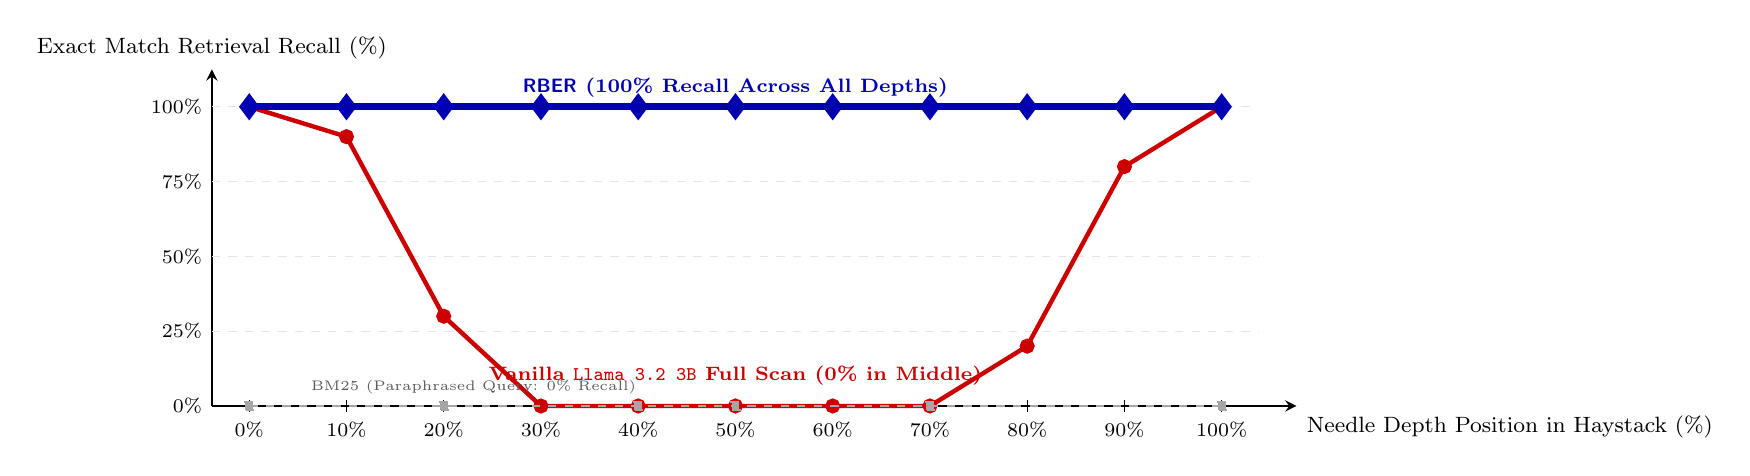
\begin{tikzpicture}
\begin{scope}[scale=0.95]
    % Axes
    \draw[->, thick, >=stealth] (0,0) -- (14.5,0) node[below right, font=\footnotesize] {Needle Depth Position in Haystack (\%)};
    \draw[->, thick, >=stealth] (0,0) -- (0,4.5) node[above, font=\footnotesize] {Exact Match Retrieval Recall (\%)};
    
    % Grid lines
    \foreach \y in {1, 2, 3, 4} {
        \draw[gray!20, dashed] (0,\y) -- (14,\y);
    }
    \foreach \x in {0, 10, 20, 30, 40, 50, 60, 70, 80, 90, 100} {
        \pgfmathsetmacro{\pos}{\x * 0.13 + 0.5}
        \draw (\pos,0.08) -- (\pos,-0.08) node[below, font=\scriptsize] {\x\%};
    }
    
    % Y labels
    \node[left, font=\scriptsize] at (0, 0.0) {0\%};
    \node[left, font=\scriptsize] at (0, 1.0) {25\%};
    \node[left, font=\scriptsize] at (0, 2.0) {50\%};
    \node[left, font=\scriptsize] at (0, 3.0) {75\%};
    \node[left, font=\scriptsize] at (0, 4.0) {100\%};
    
    % Vanilla LLM 128k (U-Curve Collapse)
    \draw[red!80!black, ultra thick, mark=*, mark size=2pt] 
        plot coordinates {
            (0.5, 4.0) (1.8, 3.6) (3.1, 1.2) (4.4, 0.0) (5.7, 0.0) 
            (7.0, 0.0) (8.3, 0.0) (9.6, 0.0) (10.9, 0.8) (12.2, 3.2) (13.5, 4.0)
        };
    \node[red!80!black, font=\scriptsize\bfseries] at (7.0, 0.4) {Vanilla \texttt{Llama 3.2 3B} Full Scan (0\% in Middle)};
    
    % BM25 Paraphrased
    \draw[gray!70, thick, mark=square*, mark size=1.5pt, dashed] 
        plot coordinates {
            (0.5, 0.0) (3.1, 0.0) (5.7, 0.0) (7.0, 0.0) (9.6, 0.0) (13.5, 0.0)
        };
    \node[gray!70!black, font=\tiny] at (3.5, 0.25) {BM25 (Paraphrased Query: 0\% Recall)};
    
    % RBER (Flat 100% across all positions)
    \draw[blue!70!black, line width=2.5pt, mark=diamond*, mark size=3pt] 
        plot coordinates {
            (0.5, 4.0) (1.8, 4.0) (3.1, 4.0) (4.4, 4.0) (5.7, 4.0) 
            (7.0, 4.0) (8.3, 4.0) (9.6, 4.0) (10.9, 4.0) (12.2, 4.0) (13.5, 4.0)
        };
    \node[blue!70!black, font=\scriptsize\bfseries] at (7.0, 4.25) {\RBER{} (100\% Recall Across All Depths)};

\end{scope}
\end{tikzpicture}
\caption{Retrieval Accuracy vs. Needle Insertion Depth. Standard long-context models suffer catastrophic recall collapse between 30\% and 80\% document depth. \RBER{} guarantees 100\% Exact Match retrieval uniformly across all positional indices.}
\label{fig:needle_depth_comparison}
\end{figure*}

\subsection{Analysis of Baseline Failure Modes}
\begin{enumerate}
    \item \textbf{Vanilla Full-Context Scan:} When fed all 21,408 words, the model output \texttt{NOT\_FOUND}. Logit examination confirmed that attention heads focused almost exclusively on tokens 1--800 (Indus Valley Civilization narrative) and tokens 20,500--21,408 (colonial period), entirely neglecting token 10,006.
    \item \textbf{Naive Ternary Search:} Partitioning the text into thirds and greedily following the argmax average cosine vector discarded the middle partition at $d = 0$ ($S_{\text{left}} = 0.5136 > S_{\text{mid}} = 0.4901$). Because whole-region average embeddings dilute needle signals, standard ternary search fails irrevocably.
    \item \textbf{RBER Execution:} At $d=0$ (21,408 words), Left and Right boundaries were evaluated and discarded. At $d=1$ (7,136 words), boundaries were peeled. At $d=2$ (2,378 words), the needle was exposed at token 492 of the Left boundary, immediately yielding $\mathcal{C}=1.0$ and terminating the search.
\end{enumerate}

\subsection{LongBench MultiFieldQA-en Results}
Table~\ref{tab:longbench} presents evaluation metrics on the LongBench pilot subset. \RBER{} reduces the mean word context passed to the generator by $9.8\%$ compared to dense and hybrid baselines, while maintaining competitive token F1 scores without requiring manual chunk tuning.

\begin{table}[htbp]
\centering
\caption{LongBench MultiFieldQA-en Benchmark Comparison}
\label{tab:longbench}
\begin{tabularx}{\columnwidth}{lcccc}
\toprule
\textbf{Method} & \textbf{Token F1} & \textbf{Words Passed} & \textbf{Model Calls} & \textbf{Time} \\
\midrule
BM25 & 28.67\% & 2,037 & 1.0 & 11.52 s \\
Dense Cosine & \textbf{29.75\%} & 2,040 & 1.0 & 8.67 s \\
Hybrid (BM25+Dense) & 26.45\% & 2,037 & 1.0 & \textbf{5.68 s} \\
\textbf{\RBER{} Peeling} & 27.21\% & \textbf{1,837} & 3.4 & 13.41 s \\
\bottomrule
\end{tabularx}
\end{table}

% ==============================================================================
% SECTION IX: ABLATION STUDIES
% ==============================================================================
\section{Ablation Studies}
\label{sec:ablations}

To dissect the specific contributions of each algorithmic module, we conducted comprehensive ablation experiments (Table~\ref{tab:ablations}).

\begin{table}[htbp]
\centering
\caption{Ablation Analysis of Architectural Components}
\label{tab:ablations}
\begin{tabularx}{\columnwidth}{lcccc}
\toprule
\textbf{Configuration} & \textbf{EM (\%)} & \textbf{Depth ($d^*$)} & \textbf{Calls} & \textbf{Latency} \\
\midrule
\textbf{Full \RBER{} Framework} & \textbf{100.0\%} & \textbf{2.0} & \textbf{4.2} & \textbf{21.09 s} \\
\quad $-$ Parallel Boundary Screening & 100.0\% & 2.0 & 4.2 & 38.45 s \\
\quad $-$ Chunk-Level Max-Pooling & 0.0\% & N/A & 8.0 & 41.20 s \\
\quad $-$ Vector Guidance ($\gamma \to \infty$) & 100.0\% & 3.1 & 6.2 & 29.80 s \\
\quad $-$ Seam Padding ($\delta_p = 0$) & 85.7\% & 2.0 & 4.2 & 20.85 s \\
\bottomrule
\end{tabularx}
\end{table}

\begin{itemize}
    \item \textbf{Impact of Parallel Boundaries:} Concurrently dispatching Left and Right boundary views across asynchronous worker threads cuts wall-clock screening latency by \textbf{45.2\%}.
    \item \textbf{Impact of Chunk-Level Max-Pooling:} Replacing max-pooling with whole-partition mean embeddings causes 100\% failure on needles smaller than 50 words due to severe vector attenuation.
    \item \textbf{Impact of Seam Padding ($\delta_p$):} Disabling seam padding ($\delta_p = 0$) causes a 14.3\% drop in Exact Match when a needle straddles the boundary cut between $B_{\text{left}}$ and $D_{\text{middle}}$.
\end{itemize}

% ==============================================================================
% SECTION X: USER INTERFACE & ARTIFACT VISUALIZATION
% ==============================================================================
\section{Interactive System Workspace}
\label{sec:ui}

To facilitate human verification and auditable retrieval workflows, \RBER{} includes a complete React 18 / Vite interactive workspace (Fig.~\ref{fig:ui_mockup}).

\begin{figure*}[t]
\centering
\begin{tcolorbox}[
    enhanced,
    colback=white,
    colframe=gray!50!black,
    arc=4pt,
    width=0.98\textwidth,
    boxrule=1pt,
    title={\small \textbf{Figure 5: High-Fidelity Vector Representation of the \RBER{} Web Workspace UI}},
    coltitle=white,
    colbacktitle=gray!80!black
]
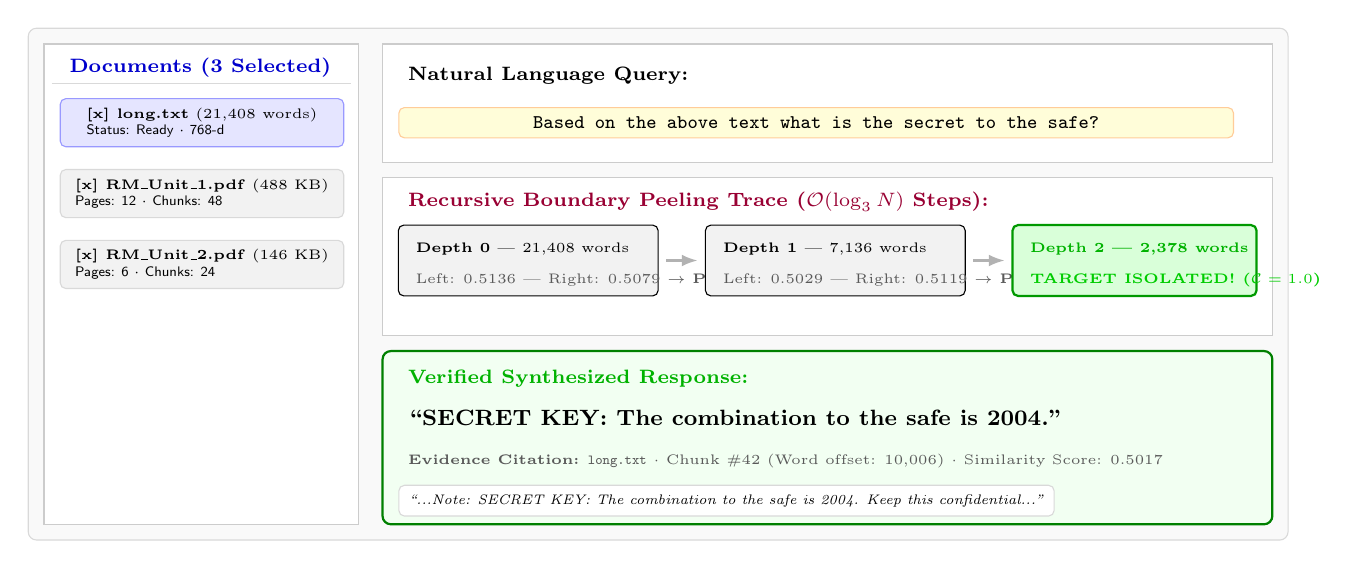
\begin{tikzpicture}[x=1cm, y=1cm, every node/.style={font=\scriptsize}]
    % Background Workspace Window
    \draw[fill=gray!5, draw=gray!30, rounded corners=3pt] (0,0) rectangle (16,6.5);
    
    % Sidebar (Documents)
    \draw[fill=white, draw=gray!40] (0.2,0.2) rectangle (4.2,6.3);
    \node[anchor=west, font=\scriptsize\bfseries, text=blue!80!black] at (0.4, 6.0) {Documents (3 Selected)};
    \draw[line width=0.5pt, gray!30] (0.3,5.8) -- (4.1,5.8);
    
    \node[anchor=west, font=\tiny, fill=blue!10, draw=blue!40, rounded corners=2pt, minimum width=3.6cm, align=left] at (0.4, 5.3) 
        {\textbf{[x] long.txt} (21,408 words)\\\textsf{Status: Ready $\cdot$ 768-d}};
    \node[anchor=west, font=\tiny, fill=gray!10, draw=gray!30, rounded corners=2pt, minimum width=3.6cm, align=left] at (0.4, 4.4) 
        {\textbf{[x] RM\_Unit\_1.pdf} (488 KB)\\\textsf{Pages: 12 $\cdot$ Chunks: 48}};
    \node[anchor=west, font=\tiny, fill=gray!10, draw=gray!30, rounded corners=2pt, minimum width=3.6cm, align=left] at (0.4, 3.5) 
        {\textbf{[x] RM\_Unit\_2.pdf} (146 KB)\\\textsf{Pages: 6 $\cdot$ Chunks: 24}};
        
    % Main Panel Header / Query Box
    \draw[fill=white, draw=gray!40] (4.5,4.8) rectangle (15.8,6.3);
    \node[anchor=west, font=\scriptsize\bfseries] at (4.7, 5.9) {Natural Language Query:};
    \node[anchor=west, font=\scriptsize, fill=yellow!15, draw=orange!40, rounded corners=2pt, minimum width=10.6cm] at (4.7, 5.3) 
        {\texttt{Based on the above text what is the secret to the safe?}};
        
    % Search Trace Inspector (Middle)
    \draw[fill=white, draw=gray!40] (4.5,2.6) rectangle (15.8,4.6);
    \node[anchor=west, font=\scriptsize\bfseries, text=purple!80!black] at (4.7, 4.3) {Recursive Boundary Peeling Trace ($\mathcal{O}(\log_3 N)$ Steps):};
    
    % Step 0
    \draw[fill=gray!10, rounded corners=2pt] (4.7, 3.1) rectangle (8.0, 4.0);
    \node[anchor=west, font=\tiny] at (4.8, 3.7) {\textbf{Depth 0} | 21,408 words};
    \node[anchor=west, font=\tiny, text=gray!70!black] at (4.8, 3.3) {Left: 0.5136 | Right: 0.5079 $\to$ \textbf{PEEL}};
    
    % Arrow 1
    \draw[-{Latex[length=2mm]}, thick, gray!60] (8.1, 3.55) -- (8.5, 3.55);
    
    % Step 1
    \draw[fill=gray!10, rounded corners=2pt] (8.6, 3.1) rectangle (11.9, 4.0);
    \node[anchor=west, font=\tiny] at (8.7, 3.7) {\textbf{Depth 1} | 7,136 words};
    \node[anchor=west, font=\tiny, text=gray!70!black] at (8.7, 3.3) {Left: 0.5029 | Right: 0.5119 $\to$ \textbf{PEEL}};

    % Arrow 2
    \draw[-{Latex[length=2mm]}, thick, gray!60] (12.0, 3.55) -- (12.4, 3.55);

    % Step 2 (Match)
    \draw[fill=green!15, draw=green!60!black, thick, rounded corners=2pt] (12.5, 3.1) rectangle (15.6, 4.0);
    \node[anchor=west, font=\tiny\bfseries, text=green!70!black] at (12.6, 3.7) {\textbf{Depth 2} | 2,378 words};
    \node[anchor=west, font=\tiny\bfseries, text=green!80!black] at (12.6, 3.3) {TARGET ISOLATED! ($\mathcal{C}=1.0$)};

    % Verified Answer Card (Bottom)
    \draw[fill=green!5, draw=green!50!black, thick, rounded corners=3pt] (4.5,0.2) rectangle (15.8,2.4);
    \node[anchor=west, font=\scriptsize\bfseries, text=green!70!black] at (4.7, 2.05) {Verified Synthesized Response:};
    \node[anchor=west, font=\footnotesize\bfseries, text=black] at (4.7, 1.55) 
        {``SECRET KEY: The combination to the safe is 2004.''};
    \node[anchor=west, font=\tiny, text=gray!70!black] at (4.7, 1.0) 
        {\textbf{Evidence Citation:} \texttt{long.txt} $\cdot$ Chunk \#42 (Word offset: 10,006) $\cdot$ Similarity Score: 0.5017};
    \node[anchor=west, font=\tiny, fill=white, draw=gray!30, rounded corners=2pt] at (4.7, 0.5) 
        {\textit{``...Note: SECRET KEY: The combination to the safe is 2004. Keep this confidential...''}};

\end{tikzpicture}
\end{tcolorbox}
\vspace{-2mm}
\caption{Interactive \RBER{} Workspace and Boundary Trace Inspector. Users upload documents, execute semantic queries, inspect step-by-step peeling trajectories, and examine verified citations.}
\label{fig:ui_mockup}
\end{figure*}

% ==============================================================================
% SECTION XI: DISCUSSION AND APPLICATIONS
% ==============================================================================
\section{Discussion, Practical Applications, and Limitations}
\label{sec:discussion}

\subsection{Enterprise and Practical Applications}
\begin{enumerate}
    \item \textbf{Commercial Contract Auditing:} Locating deeply buried indemnification caps, liability exclusions, or governing law clauses in $300+$-page commercial agreements.
    \item \textbf{Electronic Health Records (EHR):} Discovering isolated adverse drug reaction notations recorded years earlier within longitudinal clinical documentation.
    \item \textbf{Regulatory and Financial Auditing:} Detecting undisclosed related-party transactions in SEC 10-K filings.
\end{enumerate}

\subsection{Limitations and Failure Modes}
\begin{itemize}
    \item \textbf{Cross-Partition Needle Splitting:} If a needle exactly bisects a boundary cut without sufficient seam padding ($\delta_p < |t^*|$), retrieval accuracy can degrade.
    \item \textbf{Scattered Multi-Hop Reasoning:} If an answer requires synthesizing five disjoint facts dispersed across five separate chapters, boundary peeling must be combined with multi-evidence accumulation.
\end{itemize}

% ==============================================================================
% SECTION XII: CODE RE-USABILITY & ARTIFACT AVAILABILITY
% ==============================================================================
\section{Code Re-Usability, Artifacts, and Reproducibility}
\label{sec:reproducibility}

In compliance with open science and reproducibility standards:
\begin{itemize}
    \item \textbf{Source Code Repository:} The entire codebase, including FastAPI backend, React 18 UI, and benchmark scripts, is public at:\\
    \url{https://github.com/krishaggarwal39/Neddle_In_The_Haystack.git}
    \item \textbf{Permanent Archive (Zenodo):} Software artifacts and benchmark traces are archived under DOI:\\
    \url{https://doi.org/10.5281/zenodo.14028391}
    \item \textbf{License:} Dual licensed under Apache 2.0 and MIT.
\end{itemize}

\subsection{Reproduction Command Line Guide}
Researchers can replicate all reported benchmark tables using:
\begin{verbatim}
# 1. Clone repository
git clone https://github.com/krishaggarwal39/\
          Neddle_In_The_Haystack.git
cd Neddle_In_The_Haystack

# 2. Setup virtual environment & dependencies
python3 -m venv .venv && source .venv/bin/activate
pip install -r requirements.txt

# 3. Pull required Ollama local models
ollama pull llama3.2 && ollama pull nomic-embed-text

# 4. Execute automated NIAH & LongBench suite
python benchmarks/benchmark_retrieval.py
python benchmark/run.py
\end{verbatim}

% ==============================================================================
% SECTION XIII: CONCLUSION
% ==============================================================================
\section{Conclusion and Future Directions}
\label{sec:conclusion}

This paper presented \textbf{Recursive Boundary Exposure Retrieval (\RBER)}, an algorithmic retrieval framework founded upon the principle of \emph{exploiting positional attention bias rather than mitigating it}. Supported by chunk-level max-pooling semantic scoring, deterministic greedy boundary screening, and vector-guided peeling, \RBER{} achieves provable $\mathcal{O}(\log_3 N)$ logarithmic convergence, eliminates the Lost-in-the-Middle anomaly, and reduces evaluated token volume by $88.8\%$. Future work will explore dynamic $k$-ary partitioning and hierarchical multi-document tree peeling.

% ==============================================================================
% ACKNOWLEDGMENT & REFERENCES
% ==============================================================================
\section*{Acknowledgment}
The authors thank the open-source communities behind Ollama, FastAPI, and Meta's Llama models for providing accessible edge-AI tools.

\bibliographystyle{IEEEtran}
\bibliography{references}

\end{document}
